\documentclass[
11pt, % The default document font size, options: 10pt, 11pt, 12pt
%codirector, % Uncomment to add a codirector to the title page
]{charter} 




% El títulos de la memoria, se usa en la carátula y se puede usar el cualquier lugar del documento con el comando \ttitle
\titulo{Monitoreo de un Túnel de Congelado} 

% Nombre del posgrado, se usa en la carátula y se puede usar el cualquier lugar del documento con el comando \degreename
%\posgrado{Carrera de Especialización en Sistemas Embebidos} 
\posgrado{Carrera de Especialización en Internet de las Cosas} 
%\posgrado{Carrera de Especialización en Intelegencia Artificial}
%\posgrado{Maestría en Sistemas Embebidos} 
%\posgrado{Maestría en Internet de las cosas}

% Tu nombre, se puede usar el cualquier lugar del documento con el comando \authorname
\autor{Lic. Leandro Ciribé}

% El nombre del director y co-director, se puede usar el cualquier lugar del documento con el comando \supname y \cosupname y \pertesupname y \pertecosupname
\director{Mg. Ing. Marcelo Pistarelli}
\pertenenciaDirector{UNR} 
% FIXME:NO IMPLEMENTADO EL CODIRECTOR ni su pertenencia
\codirector{John Doe} % para que aparezca en la portada se debe descomentar la opción codirector en el documentclass
\pertenenciaCoDirector{FIUBA}

% Nombre del cliente, quien va a aprobar los resultados del proyecto, se puede usar con el comando \clientename y \empclientename
\cliente{Edgar A. Ciribé }
\empresaCliente{Edgar A. Ciribé S.A. }

% Nombre y pertenencia de los jurados, se pueden usar el cualquier lugar del documento con el comando \jurunoname, \jurdosname y \jurtresname y \perteunoname, \pertedosname y \pertetresname.
\juradoUno{Nombre y Apellido (1)}
\pertenenciaJurUno{pertenencia (1)} 
\juradoDos{Nombre y Apellido (2)}
\pertenenciaJurDos{pertenencia (2)}
\juradoTres{Nombre y Apellido (3)}
\pertenenciaJurTres{pertenencia (3)}
 
\fechaINICIO{30 de abril de 2021}		%Fecha de inicio de la cursada de GdP \fechaInicioName
\fechaFINALPlan{18 de junio de 2021} 	%Fecha de final de cursada de GdP
\fechaFINALTrabajo{15 de mayo de 2022}	%Fecha de defensa pública del trabajo final


\begin{document}

\maketitle
\thispagestyle{empty}
\pagebreak


\thispagestyle{empty}
{\setlength{\parskip}{0pt}
\tableofcontents{}
}
\pagebreak


\section{Registros de cambios}
\label{sec:registro}


\begin{table}[ht]
\label{tab:registro}
\centering
\begin{tabularx}{\linewidth}{@{}|c|X|c|@{}}
\hline
\rowcolor[HTML]{C0C0C0} 
Revisión & \multicolumn{1}{c|}{\cellcolor[HTML]{C0C0C0}Detalles de los cambios realizados} & Fecha      \\ \hline
0      & Creación del documento                                 &\fechaInicioName \\ \hline
1      & Se completa hasta el punto 3 inclusive                 & 13/05/2021 \\ \hline
%2      & Se completa hasta el punto 7 inclusive
%		  Se puede agregar algo más \newline
%		  En distintas líneas \newline
%		  Así                                                    & dd/mm/aaaa \\ \hline
%3      & Se completa hasta el punto 11 inclusive                & dd/mm/aaaa \\ \hline
%4      & Se completa el plan	                                 & dd/mm/aaaa \\ \hline
\end{tabularx}
\end{table}

\pagebreak



\section{Acta de constitución del proyecto}
\label{sec:acta}

\begin{flushright}
Santa Fe, \fechaInicioName
\end{flushright}

\vspace{2cm}

Por medio de la presente se acuerda con el \authorname\hspace{1px} que su Trabajo Final de la \degreename\hspace{1px} se titulará ``\ttitle'', consistirá esencialmente en el sensado de parámetros útiles para obtener la información que permita identificar, predecir y alertar ante cualquier desvío o falla técnica, maximizando la disponibilidad de la central de frío, y tendrá un presupuesto preliminar estimado de 600 hs de trabajo y {\$40.000}, con fecha de inicio \fechaInicioName\hspace{1px} y fecha de presentación pública \fechaFinalName.

Se adjunta a esta acta la planificación inicial.

\vfill

% Esta parte se construye sola con la información que hayan cargado en el preámbulo del documento y no debe modificarla
\begin{table}[ht]
\centering
\begin{tabular}{ccc}
\begin{tabular}[c]{@{}c@{}}Ariel Lutenberg \\ Director posgrado FIUBA\end{tabular} & \hspace{2cm} & \begin{tabular}[c]{@{}c@{}}\clientename \\ \empclientename \end{tabular} \vspace{2.5cm} \\ 
\multicolumn{3}{c}{\begin{tabular}[c]{@{}c@{}} \supname \\ Director del Trabajo Final\end{tabular}} \vspace{2.5cm} \\
%\begin{tabular}[c]{@{}c@{}}\jurunoname \\ Jurado del Trabajo Final\end{tabular}     &  & \begin{tabular}[c]{@{}c@{}}\jurdosname\\ Jurado del Trabajo Final\end{tabular}  \vspace{2.5cm}  \\
%\multicolumn{3}{c}{\begin{tabular}[c]{@{}c@{}} \jurtresname\\ Jurado del Trabajo Final\end{tabular}} \vspace{.5cm}                                                                     
\end{tabular}
\end{table}




\section{Descripción técnica-conceptual del proyecto a realizar}
\label{sec:descripcion}

\begin{consigna}{black}

\empclientename es una empresa dedicada al procesamiento de cuartos de carne bovina con destino de consumo humano en el mercado interno y de exportación. El producto terminado se dispone en cajas que rondan los 23 kilos de peso y son almacenadas en cámaras de enfriado o congelado, dependiendo del destino final de comercialización y de los requerimientos de cada uno de sus clientes.

Para el proceso de congelado, la caja debe ingresarse en un “túnel de congelado” por 36 horas para que alcance una temperatura bajo cero y pueda ser luego trasladada a la cámara de congelado donde se almacenará a una temperatura aproximada de -24ºC.

Actualmente, el establecimiento frigorífico cuenta con un sistema de monitoreo y alertas de gran parte de sus instalaciones de frío; entre las cuales se incluyen el sensado de temperatura ambiente de todas las cámaras de la planta, el monitoreo de encendido y apagado de las mismas y el control de la central de congelado. Para toda esta implementación se utilizó hardware de sensado basado en el controlador WiFi ESP8266 y una gran integración de distintos sistemas de software para la visualización de los valores en tiempo real y el almacenamiento de los datos recolectados para su posterior análisis. Para el sistema de alertas se utiliza el correo electrónico, dado que es el medio más efectivo para el personal de mantenimiento.

El presente proyecto se destaca especialmente por incorporar al sistema actual el monitoreo del túnel de congelado, que es una de las actividades claves en el proceso de conservación y almacenamiento de la carne con destino a exportación, como se puede observar en la figura \ref{fig:canvasdone} dentro del modelo Canvas. 

\begin{figure}[htpb]
\centering 
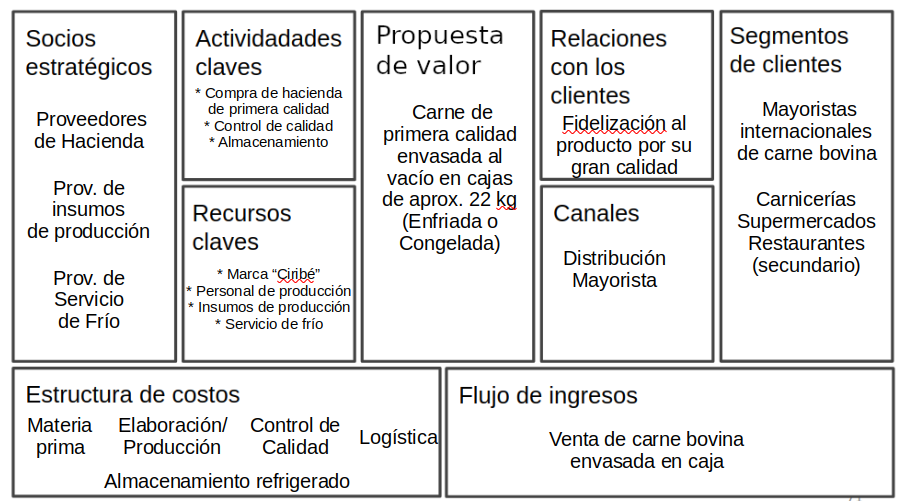
\includegraphics[width=.75\textwidth]{./Figuras/canvasdone.png}
\caption{Modelo Canvas}
\label{fig:canvasdone}
\end{figure}

Comprendiendo la importancia de suministrar alimentos seguros y saludables, la Dirección de la Empresa, toma el compromiso de implementar y mantener un sistema de Control de Calidad basado en los lineamientos del Sistema de Análisis de Riesgos y Puntos Críticos de Control (HACCP), para todos sus productos. Debido a esto, el control de temperatura tanto de carnes como de cámaras de almacenamiento, juega un papel fundamental. Además, al ser una central frigorífica con casi 22 años de edad, es imperioso contar con un sistema de monitoreo en tiempo real de las instalaciones críticas para poder predecir anomalías que pueden ser de un costo muy significativo para la empresa y su misión.

En cuanto a la parte técnica, la central de frío del túnel de congelado consta de dos compresores alemanes marca Bock de 25 hp, un banco de condensadores, dos placas de intercambio y un circuito con una bomba de circulación de agua y glicol que enfría las placas de congelamiento por contacto. Como se puede observar en la figura \ref{fig:circuito_tunel}, la central de refrigeración realiza su ciclo normal de enfriado con el objetivo de llevar el líquido circulante a temperaturas bajo cero, mientras es conducido hacia las estanterías de congelado por contacto.

\begin{figure}[htpb]
\centering 
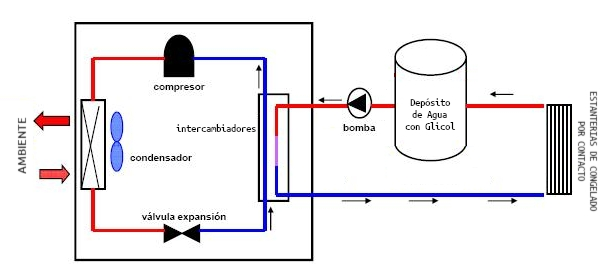
\includegraphics[width=.7\textwidth]{./Figuras/circuito_tunel.png}
\caption{Ciclo de refrigeración con depósito de agua y glicol}
\label{fig:circuito_tunel}
\end{figure}

A nivel general, el sistema debe poder cumplir con el objetivo de predecir fallas y alertar ante situaciones críticas que surjan del monitoreo de la central y, de esta manera, lograr reducir los costos de mantenimiento prolongando el tiempo de uso de los equipos. Para poder cumplir con estos requerimientos se necesitan medir los siguientes puntos:
\begin{itemize}
	\item Consumo en Amperes de cada compresor,
	\item Temperatura de succión y de salida de cada compresor,
	\item Temperatura de los intercambiadores,	
	\item Temperatura de retorno del banco de condensadores,
	\item Consumo en Amperes de la bomba de agua,
	\item Temperatura de cada estantería de congelado por contacto,
	\item Temperatura ambiente del túnel de congelado, y
	\item Temperatura exterior (ambiental).
\end{itemize}

Cada uno de estos puntos de sensado proporciona datos que pueden ser transformados en información extremadamente útil. Por ejemplo, una temperatura de succión muy baja, por un período de tiempo prolongado, puede indicar que está retornando líquido al compresor, lo cual es de una gravedad considerable.

Siguiendo el comportamiento del sistema que ya ha sido implementado parcialmente por la empresa (ver figura \ref{fig:diagramabloques}), la información recolectada por el hardware de monitoreo debe enviarse por WiFi al servidor Blynk a través del protocolo MQTT. El servidor Blynk presenta una API REST para que los datos puedan ser accedidos desde Python y almacenados en una base de datos PostgreSQL para su posterior utilización y análisis. Al momento de ir sensando y recolectando cada dato se ejecutan las validaciones correspondientes que activan alertas por correo electrónico al personal de mantenimiento. A su vez, los usuarios pueden visualizar los datos en tiempo real desde la aplicación en Blynk, ya sea dentro o fuera de la empresa, en cuyo caso la conexión se realiza a través de una red privada virtual (VPN). Para consultar, visualizar o graficar la información recolectada se utilizan páginas web en Django; y en determinados puntos críticos de control se puede acceder a información histórica específica a través de web services.

\begin{figure}[htpb]
\centering 
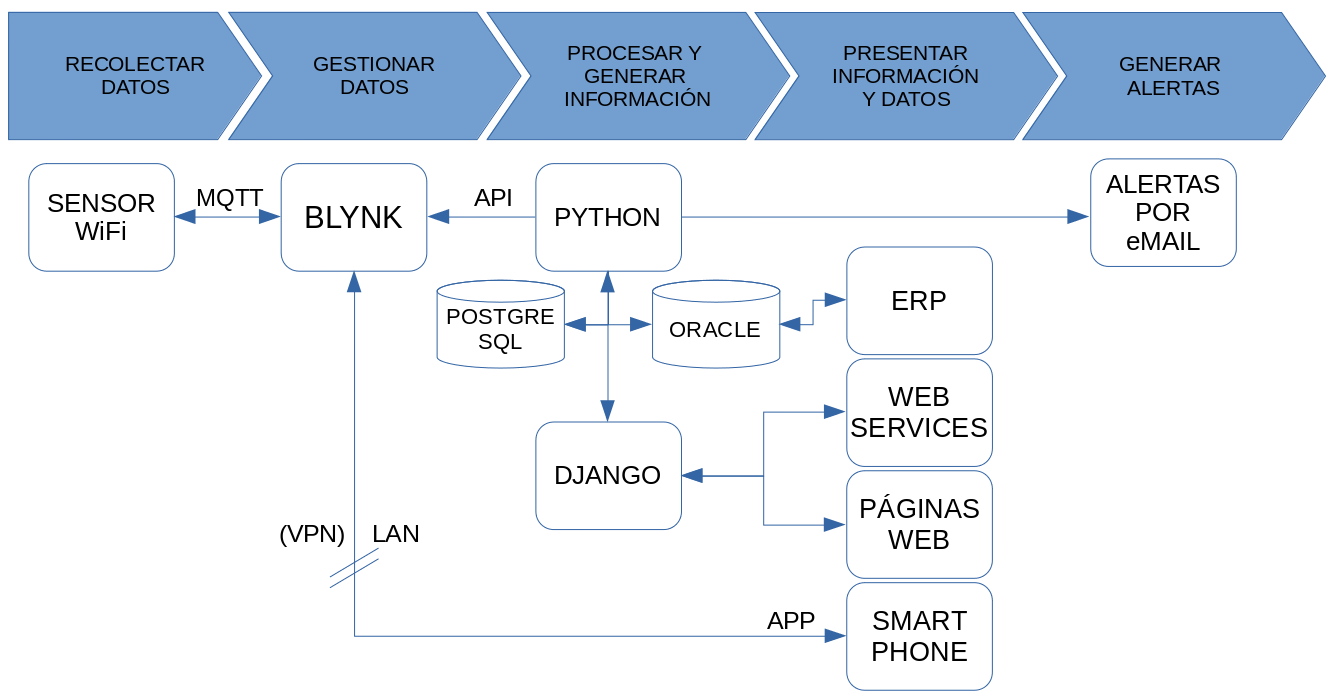
\includegraphics[width=.9\textwidth]{./Figuras/diagramabloques.png}
\caption{Diagrama de bloques del sistema}
\label{fig:diagramabloques}
\end{figure}

\end{consigna}

\section{Identificación y análisis de los interesados}
\label{sec:interesados}

\begin{consigna}{black}
A continuación se pueden observar las personas interesadas en este proyecto y el rol que cada una va a desempeñar.
\begin{table}[ht]
%\caption{Identificación de los interesados}
%\label{tab:interesados}
\begin{tabularx}{\linewidth}{@{}|l|X|X|l|@{}}
\hline
\rowcolor[HTML]{C0C0C0} 
Rol           & Nombre y Apellido & Organización 	& Puesto 	\\ \hline
Auspiciante   & \clientename      &\empclientename	& Presidente 	\\ \hline
Cliente       & \clientename      &\empclientename	&Presidente 		\\ \hline
Impulsor      & Hernán Ciribé	 &\empclientename	&Gerente Gral.		\\ \hline
Responsable   & \authorname       & FIUBA        	& Alumno 	\\ \hline
Colaboradores & Andrés Giacomino  &YACO Refrigeración 	&Dueño       	\\ \hline
Orientador    & \supname	      & \pertesupname 	& Director Trabajo final \\ \hline
Equipo        & Lucas Tondo \newline 
				Ignacio Abendaño          &\empclientename &Operarios Mantenimiento        	\\ \hline
Usuario final &Lucas Tondo \newline 
				Ignacio Abendaño \newline 
				Hernán Ciribé  \newline 
				Leandro Ciribé &\empclientename	&Gerencia y Mantenimiento \\ \hline
\end{tabularx}
\end{table}

Las principales características de cada interesado son:
\begin{itemize}
	\item Auspiciante: está muy interesado en poder reducir los costos de mantenimiento. Estima realizar una inversión inferior al costo del arreglo de un compresor, que puede llegar a rondar los 40.000 pesos.
	\item Cliente: es una persona que necesita poder constatar las mejoras obtenidas, en cuanto a ahorro monetario, debido a un mantenimiento preventivo realizado correctamente y a tiempo.
	\item Impulsor: persona que está muy interesada en incorporar adelantos tecnológicos que reduzcan los costos y mejoren la operatoria de la empresa.
	\item Responsable: está muy interesado en maximizar el tiempo de disponibilidad de los equipamientos y reducir los índices de roturas particularmente en compresores.
	\item Colaboradores: es la persona indicada para ayudar a evacuar cualquier duda sobre tecnologías de centrales frigoríficas. Tener en cuenta que a veces su tiempo disponible es escaso.
	\item Orientador: es una persona idónea para consultar y definir los objetivos a seguir en el proyecto.
	\item Equipo: ambas personas son responsables y proactivas en incorporar nuevas tecnologías que mejoren su trabajo.
	\item Usuario Final: están urgidos en disponer de la información para poder tomar las mejores decisiones dentro de su área de trabajo.
\end{itemize}
%Cliente
%Quien aprobará el producto, servicio o resultado del proyecto.
%Auspiciante
%Quien financia el proyecto y por lo tanto es la última autoridad.
%Usuario final
%Quien utilizará realmente el producido del proyecto (end user).
%Impulsor
%Una alta autoridad que hará “campaña” por el proyecto (champion).
%Orientadores
%Participan en definir los objetivos del proyecto (drivers).
%Colaboradores
%Colaboran con el proyecto y aportan recursos (supporters).
%Responsable
%Persona con autoridad para gestionar el proyecto (project manager).
%Equipo
%Las personas que harán el trabajo cotidiano del proyecto.
%Opositor
%Quien se opone a que se haga el proyecto y trata de sabotearlo
\end{consigna}



\section{1. Propósito del proyecto}
\label{sec:proposito}

\begin{consigna}{black}
El propósito de este proyecto es disponer de información útil para identificar cambios en el comportamiento normal de una central de frío, poder aprender a predecir fallas que sean de un costo significativo para la empresa y maximizar el tiempo de disponibilidad de la central frigorífica.
\end{consigna}

\section{2. Alcance del proyecto}
\label{sec:alcance}

\begin{consigna}{black}
En el presente proyecto se incorporarán nuevos sensores para medir el consumo de cada compresor y sensores de temperatura en lugares claves de la central del túnel de congelado (como ya se ha detallado anteriormente en este documento). También se utilizarán datos de sensores ya existentes en el sistema y se incorporarán las líneas de código necesarias para adaptar los nuevos sensores al sistema vigente. En el proyecto no se incluye el sensado de presión, como así tampoco el monitoreo de la central de media temperatura que será implementado en una etapa posterior.
\end{consigna}


\section{3. Supuestos del proyecto}
\label{sec:supuestos}

\begin{consigna}{black}
Para el desarrollo del presente proyecto se supone que:
\begin{itemize}
	\item La empresa dispondrá de los materiales necesarios, como por ejemplo los controladores WiFi y demás sensores.
	\item El personal de mantenimiento asistirá en las tareas de instalación y conexión del hardware.
	\item El área de informática otorgará los permisos y la infraestructura necesaria para la implementación.
\end{itemize}
\end{consigna}

\section{4. Requerimientos}
\label{sec:requerimientos}

\begin{consigna}{red}
Los requerimientos deben numerarse y de ser posible estar agruparlos por afinidad, por ejemplo:

\begin{enumerate}
	\item Requerimientos funcionales
		\begin{enumerate}
			\item El sistema debe...
			\item Tal componente debe...
			\item El usuario debe poder...
		\end{enumerate}
	\item Requerimientos de documentación
		\begin{enumerate}
			\item Requerimiento 1
			\item Requerimiento 2 (prioridad menor)
		\end{enumerate}
	\item Requerimiento de testing...
	\item Requerimientos de la interfaz...
	\item Requerimientos interoperabilidad...
	\item etc...
\end{enumerate}

Leyendo los requerimientos se debe poder interpretar cómo será el proyecto y su funcionalidad.

Indicar claramente cuál es la prioridad entre los distintos requerimientos y si hay requerimientos opcionales. 

No olvidarse de que los requerimientos incluyen a las regulaciones y normas vigentes!!!

Y al escribirlos seguir las siguientes reglas:
\begin{itemize}
	\item Ser breve y conciso (nadie lee cosas largas). 
	\item Ser específico: no dejar lugar a confusiones.
	\item Expresar los requerimientos en términos que sean cuantificables y medibles.
\end{itemize}

\end{consigna}

\section{5. Historias de usuarios (\textit{Product backlog})}
\label{sec:backlog}

\begin{consigna}{red}
Descripción: En esta sección se deben incluir las historias de usuarios y su ponderación (\textit{history points}). Recordar que las historias de usuarios son descripciones cortas y simples de una característica contada desde la perspectiva de la persona que desea la nueva capacidad, generalmente un usuario o cliente del sistema. La ponderación es un número entero que representa el tamaño de la historia comparada con otras historias de similar tipo.

Se debe indicar explícitamente el criterio para calcular los \textit{story points} de cada historia
\end{consigna}

\section{6. Entregables principales del proyecto}
\label{sec:entregables}

\begin{consigna}{red}

Los entregables del proyecto son (ejemplo):

\begin{itemize}
	\item Manual de uso
	\item Diagrama de circuitos esquemáticos
	\item Código fuente del firmware
	\item Diagrama de instalación
	\item Informe final
	\item etc...
\end{itemize}

\end{consigna}

\section{7. Desglose del trabajo en tareas}
\label{sec:wbs}

\begin{consigna}{red}
El WBS debe tener relación directa o indirecta con los requerimientos.  Son todas las actividades que se harán en el proyecto para dar cumplimiento a los requerimientos. Se recomienda mostrar el WBS mediante una lista indexada:

\begin{enumerate}
\item Grupo de tareas 1
	\begin{enumerate}
	\item Tarea 1 (tantas hs)
	\item Tarea 2 (tantas hs)
	\item Tarea 3 (tantas hs)
	\end{enumerate}
\item Grupo de tareas 2
	\begin{enumerate}
	\item Tarea 1 (tantas hs)
	\item Tarea 2 (tantas hs)
	\item Tarea 3 (tantas hs)
	\end{enumerate}
\item Grupo de tareas 3
	\begin{enumerate}
	\item Tarea 1 (tantas hs)
	\item Tarea 2 (tantas hs)
	\item Tarea 3 (tantas hs)
	\item Tarea 4 (tantas hs)
	\item Tarea 5 (tantas hs)
	\end{enumerate}
\end{enumerate}

Cantidad total de horas: (tantas hs)

Se recomienda que no haya ninguna tarea que lleve más de 40 hs. 

\end{consigna}

\section{8. Diagrama de Activity On Node}
\label{sec:AoN}

\begin{consigna}{red}
Armar el AoN a partir del WBS definido en la etapa anterior. 

%La figura \ref{fig:AoN} fue elaborada con el paquete latex tikz y pueden consultar la siguiente referencia \textit{online}:

%\url{https://www.overleaf.com/learn/latex/LaTeX_Graphics_using_TikZ:_A_Tutorial_for_Beginners_(Part_3)\%E2\%80\%94Creating_Flowcharts}

\end{consigna}

\begin{figure}[htpb]
\centering 
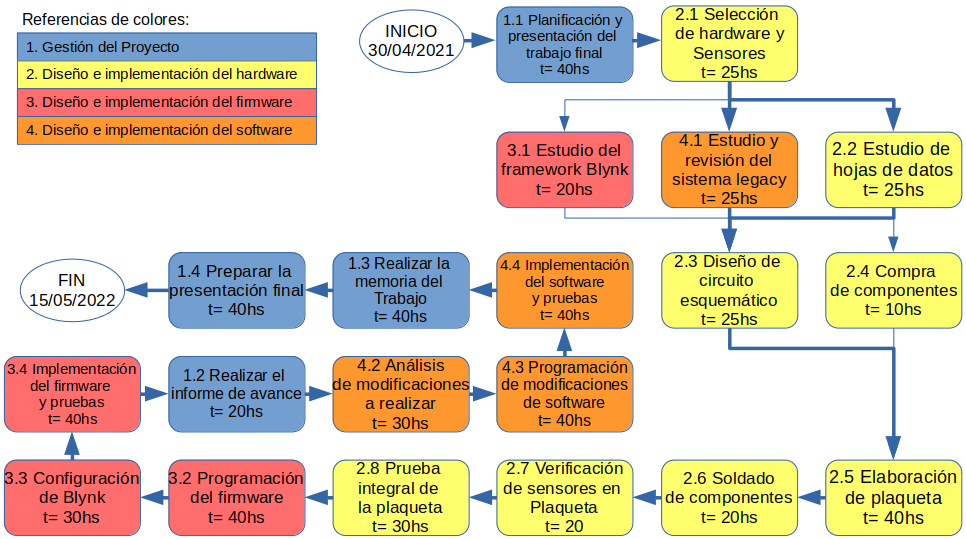
\includegraphics[width=.8\textwidth]{./Figuras/AoN.png}
\caption{Diagrama en \textit{Activity on Node}}
\label{fig:AoN}
\end{figure}

Indicar claramente en qué unidades están expresados los tiempos.
De ser necesario indicar los caminos semicríticos y analizar sus tiempos mediante un cuadro.
Es recomendable usar colores y un cuadro indicativo describiendo qué representa cada color, como se muestra en el siguiente ejemplo:



\section{9. Diagrama de Gantt}
\label{sec:gantt}

\begin{consigna}{red}

Existen muchos programas y recursos \textit{online} para hacer diagramas de gantt, entre los cuales destacamos:

\begin{itemize}
\item Planner
\item GanttProject
\item Trello + \textit{plugins}. En el siguiente link hay un tutorial oficial: \\ \url{https://blog.trello.com/es/diagrama-de-gantt-de-un-proyecto}
\item Creately, herramienta online colaborativa. \\\url{https://creately.com/diagram/example/ieb3p3ml/LaTeX}
\item Se puede hacer en latex con el paquete \textit{pgfgantt}\\ \url{http://ctan.dcc.uchile.cl/graphics/pgf/contrib/pgfgantt/pgfgantt.pdf}
\end{itemize}

Pegar acá una captura de pantalla del diagrama de Gantt, cuidando que la letra sea suficientemente grande como para ser legible. 
Si el diagrama queda demasiado ancho, se puede pegar primero la ``tabla'' del Gantt y luego pegar la parte del diagrama de barras del diagrama de Gantt.

Configurar el software para que en la parte de la tabla muestre los códigos del EDT (WBS).\\
Configurar el software para que al lado de cada barra muestre el nombre de cada tarea.\\
Revisar que la fecha de finalización coincida con lo indicado en el Acta Constitutiva.

En la figura \ref{fig:gantt}, se muestra un ejemplo de diagrama de gantt realizado con el paquete de \textit{pgfgantt}. En la plantilla pueden ver el código que lo genera y usarlo de base para construir el propio.

\begin{figure}[htbp]
\begin{center}
\begin{ganttchart}{1}{12}
  \gantttitle{2020}{12} \\
  \gantttitlelist{1,...,12}{1} \\
  \ganttgroup{Group 1}{1}{7} \\
  \ganttbar{Task 1}{1}{2} \\
  \ganttlinkedbar{Task 2}{3}{7} \ganttnewline
  \ganttmilestone{Milestone o hito}{7} \ganttnewline
  \ganttbar{Final Task}{8}{12}
  \ganttlink{elem2}{elem3}
  \ganttlink{elem3}{elem4}
\end{ganttchart}
\end{center}
\caption{Diagrama de gantt de ejemplo}
\label{fig:gantt}
\end{figure}

\end{consigna}


\section{10. Presupuesto detallado del proyecto}
\label{sec:presupuesto}

\begin{consigna}{red}
Si el proyecto es complejo entonces separarlo en partes:
\begin{itemize}
	\item Un total global, indicando el subtotal acumulado por cada una de las áreas.
	\item El desglose detallado del subtotal de cada una de las áreas.
\end{itemize}

IMPORTANTE: No olvidarse de considerar los COSTOS INDIRECTOS.

\end{consigna}

\begin{table}[htpb]
\centering
\begin{tabularx}{\linewidth}{@{}|X|c|r|r|@{}}
\hline
\rowcolor[HTML]{C0C0C0} 
\multicolumn{4}{|c|}{\cellcolor[HTML]{C0C0C0}COSTOS DIRECTOS} \\ \hline
\rowcolor[HTML]{C0C0C0} 
Descripción &
  \multicolumn{1}{c|}{\cellcolor[HTML]{C0C0C0}Cantidad} &
  \multicolumn{1}{c|}{\cellcolor[HTML]{C0C0C0}Valor unitario} &
  \multicolumn{1}{c|}{\cellcolor[HTML]{C0C0C0}Valor total} \\ \hline
 &
  \multicolumn{1}{c|}{} &
  \multicolumn{1}{c|}{} &
  \multicolumn{1}{c|}{} \\ \hline
 &
  \multicolumn{1}{c|}{} &
  \multicolumn{1}{c|}{} &
  \multicolumn{1}{c|}{} \\ \hline
\multicolumn{1}{|l|}{} &
   &
   &
   \\ \hline
\multicolumn{1}{|l|}{} &
   &
   &
   \\ \hline
\multicolumn{3}{|c|}{SUBTOTAL} &
  \multicolumn{1}{c|}{} \\ \hline
\rowcolor[HTML]{C0C0C0} 
\multicolumn{4}{|c|}{\cellcolor[HTML]{C0C0C0}COSTOS INDIRECTOS} \\ \hline
\rowcolor[HTML]{C0C0C0} 
Descripción &
  \multicolumn{1}{c|}{\cellcolor[HTML]{C0C0C0}Cantidad} &
  \multicolumn{1}{c|}{\cellcolor[HTML]{C0C0C0}Valor unitario} &
  \multicolumn{1}{c|}{\cellcolor[HTML]{C0C0C0}Valor total} \\ \hline
\multicolumn{1}{|l|}{} &
   &
   &
   \\ \hline
\multicolumn{1}{|l|}{} &
   &
   &
   \\ \hline
\multicolumn{1}{|l|}{} &
   &
   &
   \\ \hline
\multicolumn{3}{|c|}{SUBTOTAL} &
  \multicolumn{1}{c|}{} \\ \hline
\rowcolor[HTML]{C0C0C0}
\multicolumn{3}{|c|}{TOTAL} &
   \\ \hline
\end{tabularx}%
\end{table}


\section{11. Gestión de riesgos}
\label{sec:riesgos}

\begin{consigna}{red}
a) Identificación de los riesgos (al menos cinco) y estimación de sus consecuencias:
 
Riesgo 1: detallar el riesgo (riesgo es algo que si ocurre altera los planes previstos de forma negativa)
\begin{itemize}
	\item Severidad (S): mientras más severo, más alto es el número (usar números del 1 al 10).\\
	Justificar el motivo por el cual se asigna determinado número de severidad (S).
	\item Probabilidad de ocurrencia (O): mientras más probable, más alto es el número (usar del 1 al 10).\\
	Justificar el motivo por el cual se asigna determinado número de (O). 
\end{itemize}   

Riesgo 2:
\begin{itemize}
	\item Severidad (S): 
	\item Ocurrencia (O):
\end{itemize}

Riesgo 3:
\begin{itemize}
	\item Severidad (S): 
	\item Ocurrencia (O):
\end{itemize}


b) Tabla de gestión de riesgos:      (El RPN se calcula como RPN=SxO)

\begin{table}[htpb]
\centering
\begin{tabularx}{\linewidth}{@{}|X|c|c|c|c|c|c|@{}}
\hline
\rowcolor[HTML]{C0C0C0} 
Riesgo & S & O & RPN & S* & O* & RPN* \\ \hline
       &   &   &     &    &    &      \\ \hline
       &   &   &     &    &    &      \\ \hline
       &   &   &     &    &    &      \\ \hline
       &   &   &     &    &    &      \\ \hline
       &   &   &     &    &    &      \\ \hline
\end{tabularx}%
\end{table}

Criterio adoptado: 
Se tomarán medidas de mitigación en los riesgos cuyos números de RPN sean mayores a...

Nota: los valores marcados con (*) en la tabla corresponden luego de haber aplicado la mitigación.

c) Plan de mitigación de los riesgos que originalmente excedían el RPN máximo establecido:
 
Riesgo 1: plan de mitigación (si por el RPN fuera necesario elaborar un plan de mitigación).
  Nueva asignación de S y O, con su respectiva justificación:
  - Severidad (S): mientras más severo, más alto es el número (usar números del 1 al 10).
          Justificar el motivo por el cual se asigna determinado número de severidad (S).
  - Probabilidad de ocurrencia (O): mientras más probable, más alto es el número (usar del 1 al 10).
          Justificar el motivo por el cual se asigna determinado número de (O).

Riesgo 2: plan de mitigación (si por el RPN fuera necesario elaborar un plan de mitigación).
 
Riesgo 3: plan de mitigación (si por el RPN fuera necesario elaborar un plan de mitigación).

\end{consigna}


\section{12. Gestión de la calidad}
\label{sec:calidad}

\begin{consigna}{red}
Para cada uno de los requerimientos del proyecto indique:
\begin{itemize} 
\item Req \#1: copiar acá el requerimiento.

\begin{itemize}
	\item Verificación para confirmar si se cumplió con lo requerido antes de mostrar el sistema al cliente. Detallar 
	\item Validación con el cliente para confirmar que está de acuerdo en que se cumplió con lo requerido. Detallar  
\end{itemize}

\end{itemize}

Tener en cuenta que en este contexto se pueden mencionar simulaciones, cálculos, revisión de hojas de datos, consulta con expertos, mediciones, etc.  Las acciones de verificación suelen considerar al entregable como ``caja blanca'', es decir se conoce en profundidad su funcionamiento interno.  En cambio, las acciones de validación suelen considerar al entregable como ``caja negra'', es decir, que no se conocen los detalles de su funcionamiento interno.

\end{consigna}

\section{13. Procesos de cierre}    
\label{sec:cierre}

\begin{consigna}{red}
Establecer las pautas de trabajo para realizar una reunión final de evaluación del proyecto, tal que contemple las siguientes actividades:

\begin{itemize}
	\item Pautas de trabajo que se seguirán para analizar si se respetó el Plan de Proyecto original:
	 - Indicar quién se ocupará de hacer esto y cuál será el procedimiento a aplicar. 
	\item Identificación de las técnicas y procedimientos útiles e inútiles que se emplearon, y los problemas que surgieron y cómo se solucionaron:
	 - Indicar quién se ocupará de hacer esto y cuál será el procedimiento para dejar registro.
	\item Indicar quién organizará el acto de agradecimiento a todos los interesados, y en especial al equipo de trabajo y colaboradores:
	  - Indicar esto y quién financiará los gastos correspondientes.
\end{itemize}

\end{consigna}


\end{document}
